%\begin{frame}{Extraction des phrases-clés}
%\og{}\textcolor{deepblue}{Phrases-clés}\fg{}, angl. \textit{keyphrases}
%\begin{itemize}
%\item séquences de plusieurs mots (ex. \textit{sclérose latérale amyotrophique})
%\item reflètent plus précisément le contexte sémantique du texte \\\small{$\neq$ mots-clés, angl. \textit{keywords} : unigrammes de mot (ex. \textit{sclérose})}
%\end{itemize}
%\bigskip
%%\centering
%%Extraction de \og{}phrases-clés\fg{} (angl. \textit{keyphrases})
%%\\~\\
%%\begin{block}{Extraction de phrases-clés}
%%\justifying
%%Processus de \underline{sélection} automatique d'un petit ensemble de phrases les plus pertinentes à partir d'un texte donné \citep{schopf2022}.
%%\end{block}
%%\begin{block}{Prédiction de phrases-clés}
%%\justifying
%%Processus de \underline{génération} des phrases-clés qui résument parfaitement un document donné \citep{xie2023}.
%\begin{columns}[t,onlytextwidth]
%\column{.45\textwidth}
%\textcolor{violet}{Extraction}
%\justifying
%
%Processus de \underline{sélection} automatique d'un petit ensemble de phrases les plus pertinentes à partir d'un texte donné.
%\vspace{-0.2cm}
%\begin{flushright}
%\small{\citep{schopf2022}}
%\end{flushright} 
%\column{.45\textwidth}
%\textcolor{violet}{Prédiction}
%\justifying
%
%Processus de \underline{génération} des phrases-clés qui résument parfaitement un document donné.
%\vspace{0.3cm}
%\begin{flushright}
%\small{\citep{xie2023}}
%\end{flushright}
%\end{columns}%Extraction de phrases-clés
%%
%%Processus de \underline{sélection} automatique d'un petit ensemble de phrases les plus pertinentes à partir d'un texte donné \citep{schopf2022}.
%%
%%\begin{block}{Prédiction de phrases-clés}
%%\justifying
%%Processus de \underline{génération} des phrases-clés qui résument parfaitement un document donné \citep{xie2023}.
%%\end{block} 
%\end{frame}

\begin{frame}{Extraction des phrases-clés : méthode \texttt{keybert}}
\begin{enumerate}
\small
\item entrée : un document
\item tokénisation du document en phrases-clés candidates (PCC)
\item génération des plongements du doc. et des PCC par un modèle de langage
\item calcul de la similarité cosinus entre le document et les PC
\end{enumerate}
\begin{figure}
    \centering
    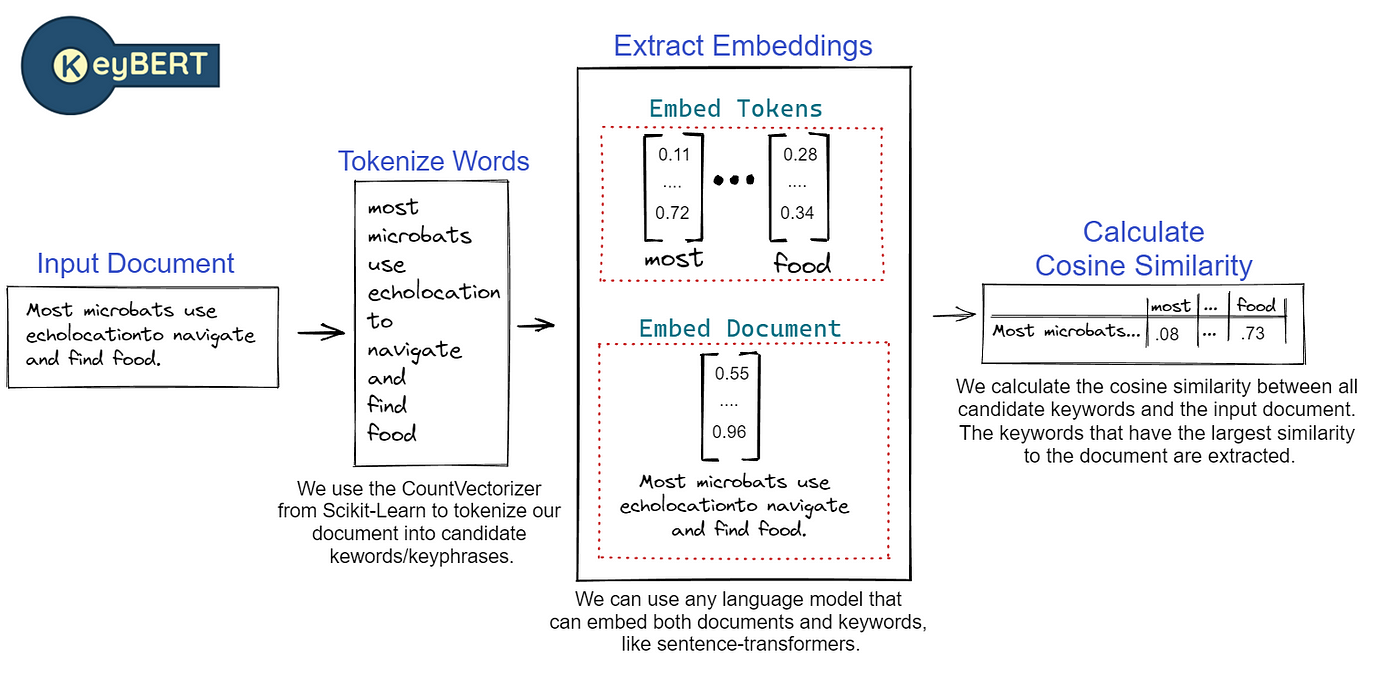
\includegraphics[width=80mm,scale=0.5]{pic/keybert.png}
    \caption{\textit{Pipeline} de la librairie \texttt{keybert} \citep{grootendorst2020keybert}.}
    \label{fig:enter-label}
\end{figure}
\end{frame}

\begin{frame}{Limitations de \texttt{keybert}}
\danger{} manque de diversification des résultats + (non-)grammaticalité\\
    \begin{figure}[!ht]
        \centering
        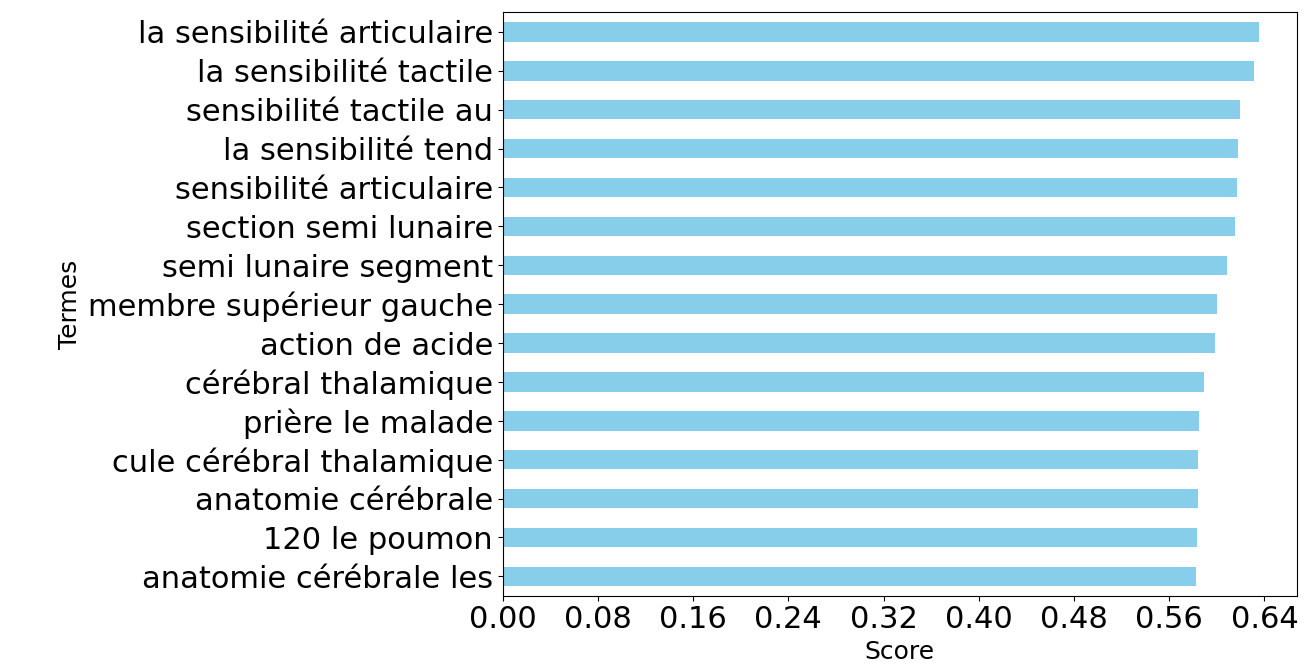
\includegraphics[width=110mm,scale=0.5]{pic/termes_keybert_autres.png}
        \caption{Répartition des 15 termes les plus pertinents dans le corpus \og{}Autres\fg{} selon \texttt{keybert}.}
        \label{fig:enter-label}
    \end{figure}
\end{frame}

\begin{frame}{Phrases-clés \textit{hapax} partagés dans les deux corpus selon \texttt{keybert}}
Les seuls termes partagés avec le corpus Charcot : 
%\begin{itemize}
%\item articulations de [\textit{sic}] épaule
%\item paralysie faciale périphérique
%\end{itemize}
    \begin{figure}[!ht]
        \centering
        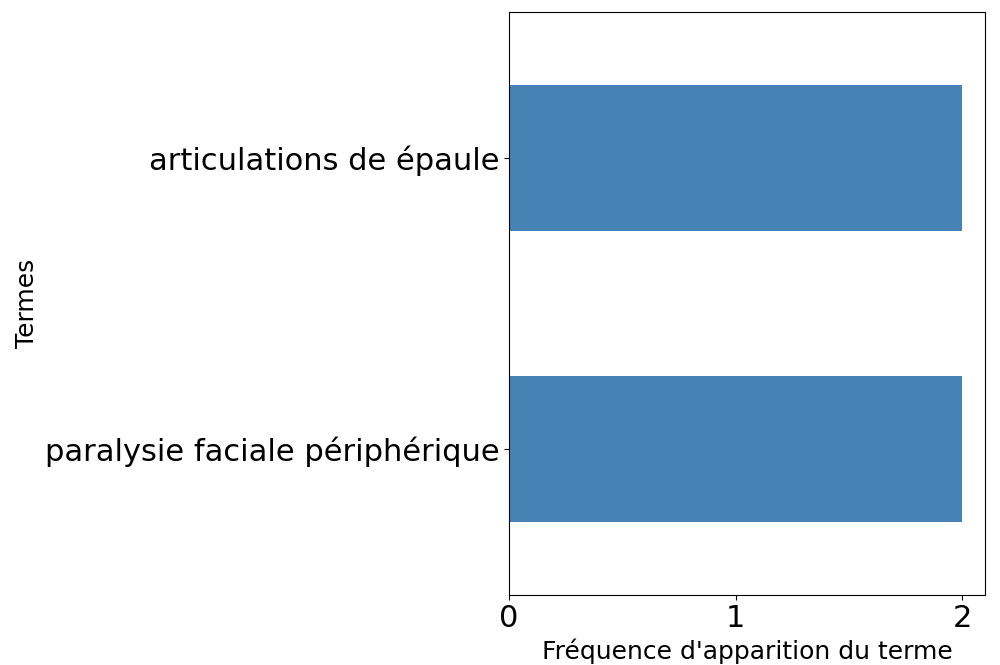
\includegraphics[width=90mm,scale=0.5]{pic/termes_partages_keybert.png}
        \caption{Répartition des termes les plus pertinents dans les deux corpus selon \texttt{keybert}.}
        \label{fig:enter-label}
    \end{figure}
\end{frame}
\begin{frame}{Extraction des phrases-clés : méthode \textit{PatternRank}\\
\quad \quad \quad\ \quad \quad \quad \quad \quad \quad \quad \ \ \ \ \ \small{Librairie \texttt{keyphrase-vectorizers}}}
%\begin{itemize}
%\item extraction des phrases-clés non-supervisée
%\item exploite des modèles de langues pré-entraînés + parties du discours
%\end{itemize}
\begin{enumerate}
\small
\item entrée : un seul document texte tokenisé
\item étiquetage des tokens avec les balises du partie du discours (POS)
\item sélection des tokens selon le motif POS $\rightarrow$ phrases-clés candidates (PCC)
\item génération des plongements du doc. et des PCC par un modèle de langue
\item calcul des similarités cosinus entre ces deux types de plongements +  \\classement des PCC par ordre décroissant
\item extraction des \textit{N} PC les plus représentatives
\end{enumerate}
\begin{figure}
    \centering
    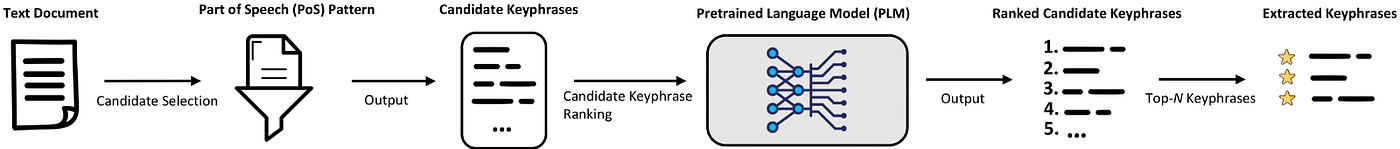
\includegraphics[width=110mm,scale=0.5]{pic/patternrank_workflow.png}
    \caption{\textit{Workflow} de la méthode \textit{PatternRank} \citep{schopf2022}.}
    \label{fig:enter-label}
\end{figure}
\notecite{schopf2022}
\end{frame}

%\begin{frame}{Termes partagés extraits avec \texttt{keyphrase-vectorizers}}
%    \begin{figure}[!ht]
%        \centering
%        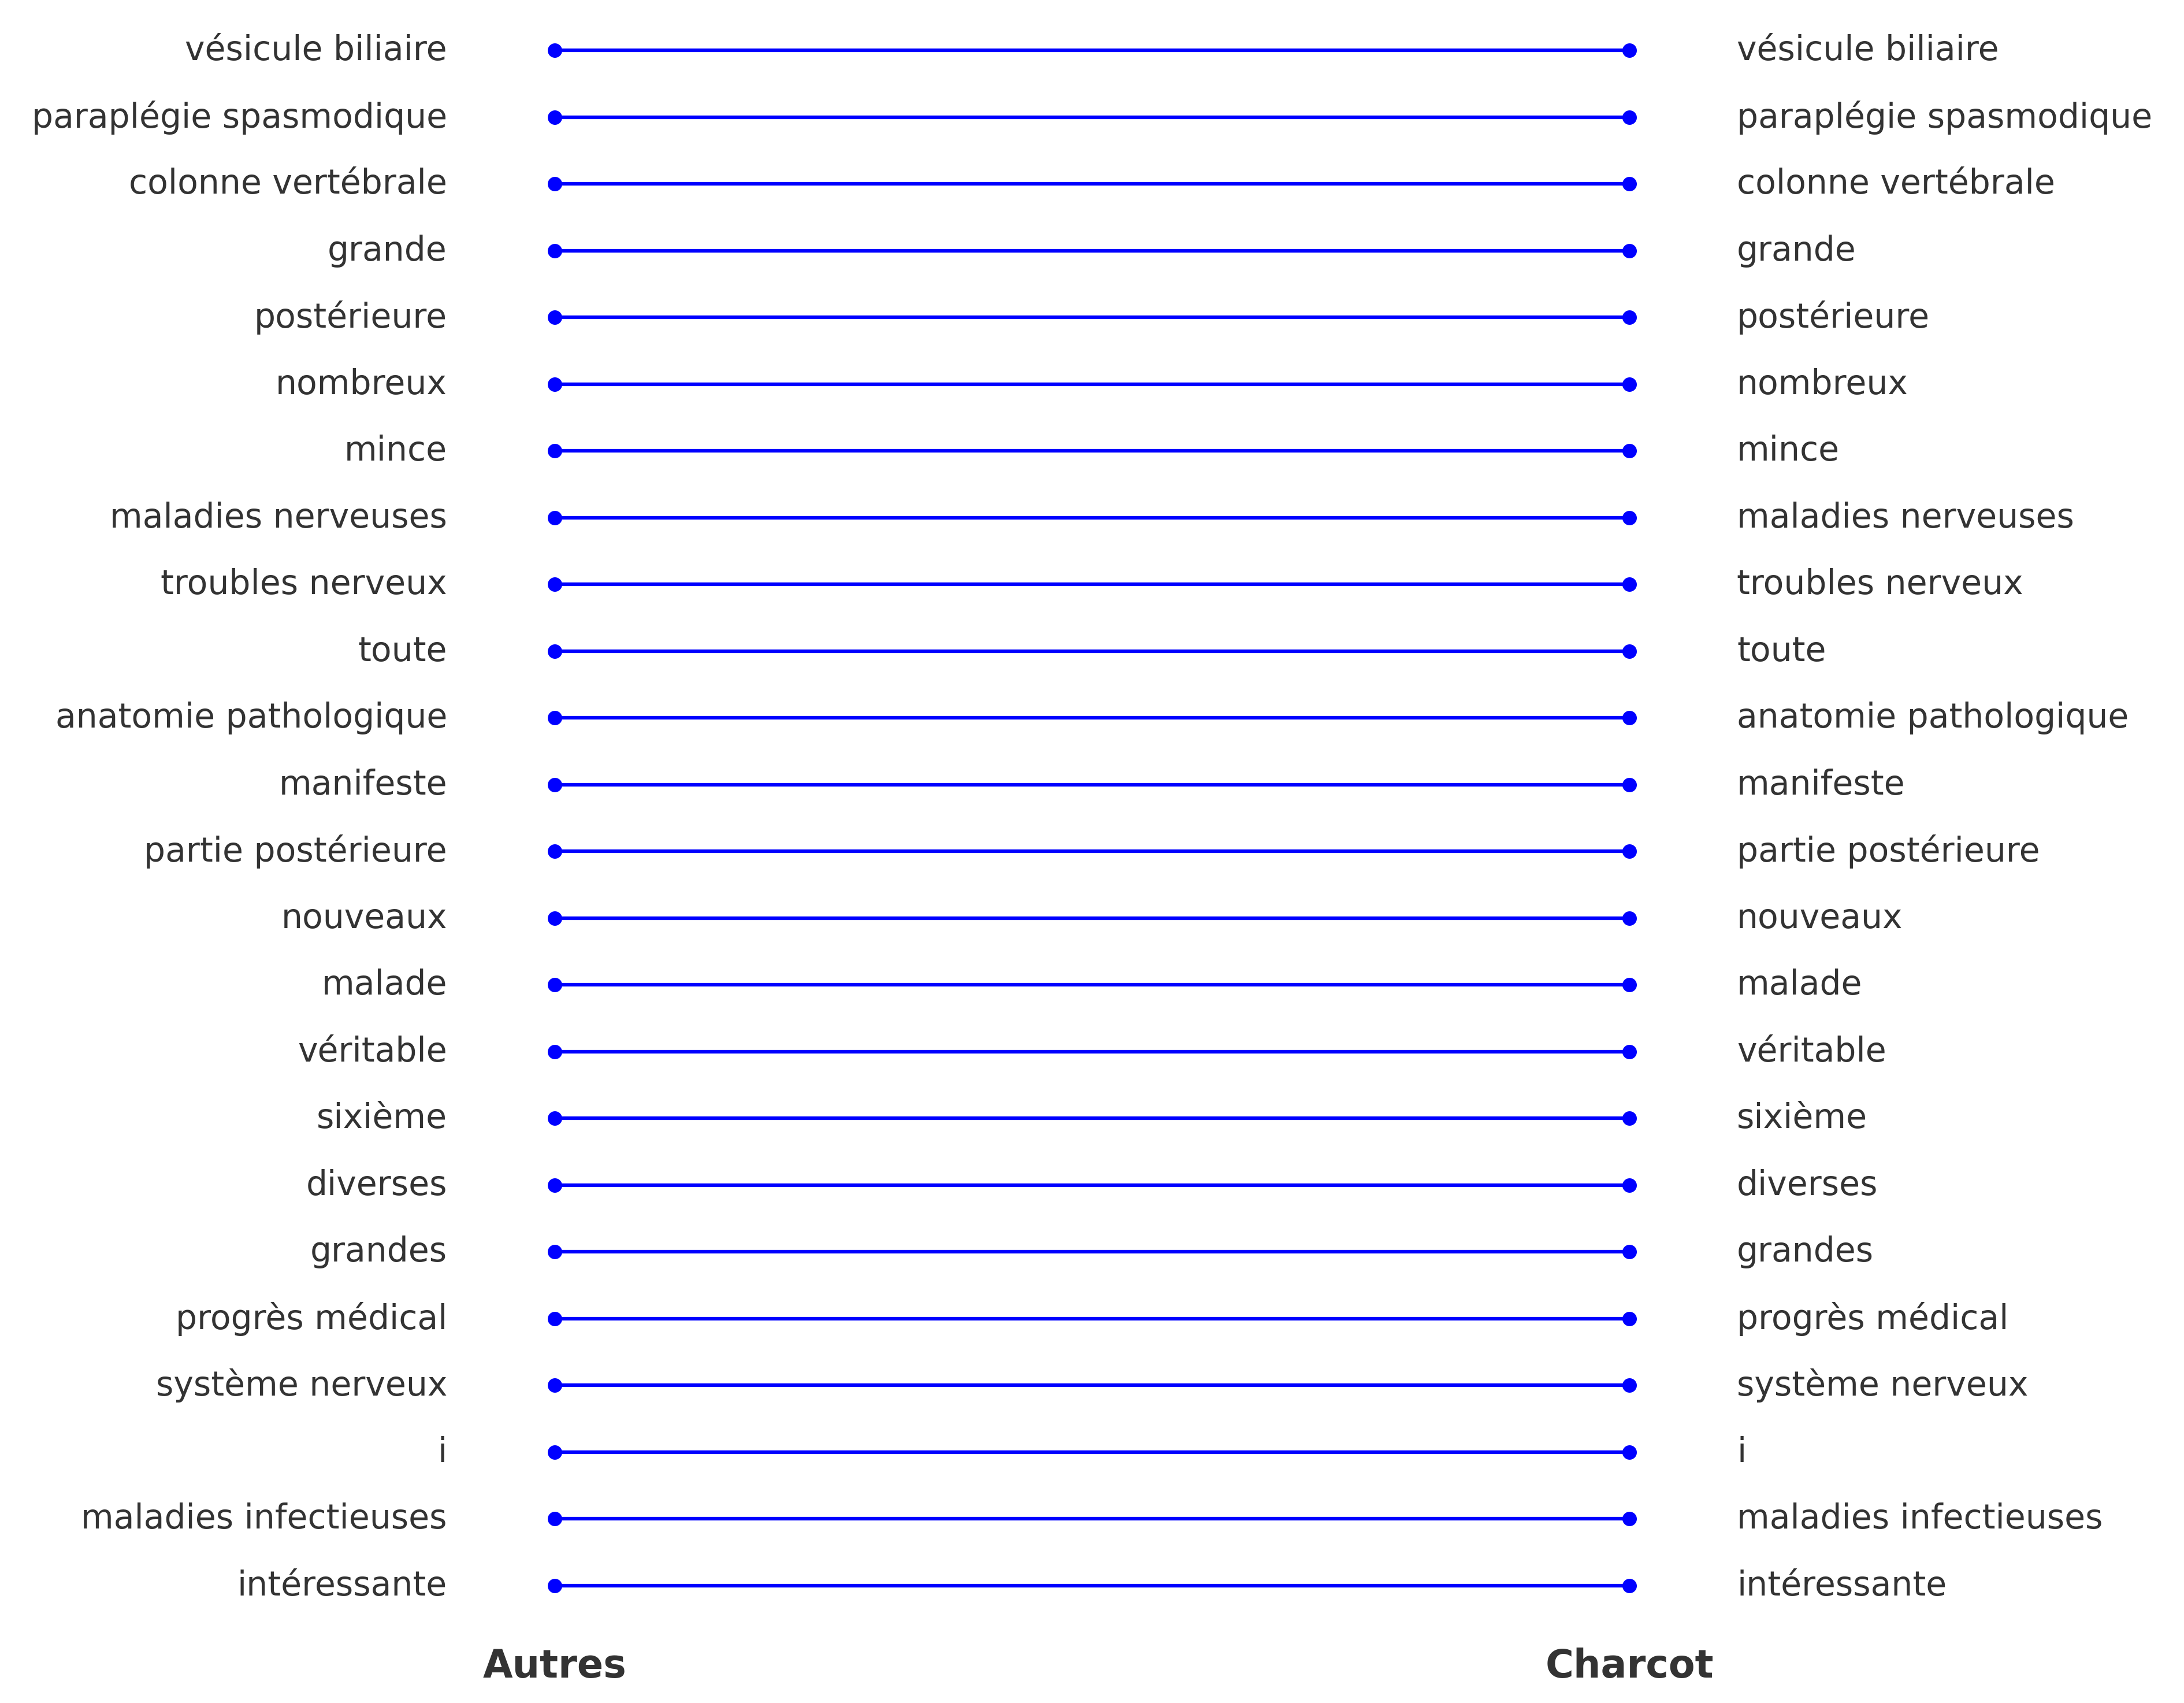
\includegraphics[width=85mm,scale=0.5]{pic/visualisation_termes_dupliques.png}
%        \caption{Les termes communs aux deux corpus selon \texttt{keyphrase-vectorizers}.}
%        \label{fig:enter-label}
%    \end{figure}
%\end{frame}

%\begin{frame}{Termes partagés | \texttt{keyphrase-vectorizers}}
%    \begin{figure}[!ht]
%        \centering
%        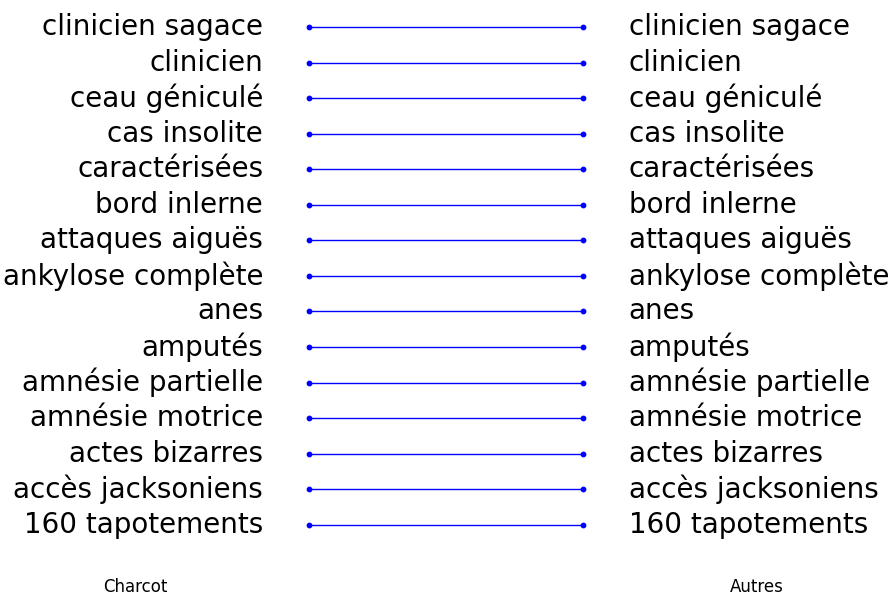
\includegraphics[width=100mm,scale=0.5]{pic/termes_partages_liens.png}
%        \caption{Les termes communs (fréq. = 1) aux deux corpus selon \texttt{keyphrase-vectorizers}.}
%        \label{fig:enter-label}
%    \end{figure}
%\end{frame}

\begin{frame}{Les termes partagés les plus fréquents | \texttt{keyphrase-vectorizers}}
    \begin{figure}[!ht]
        \centering
        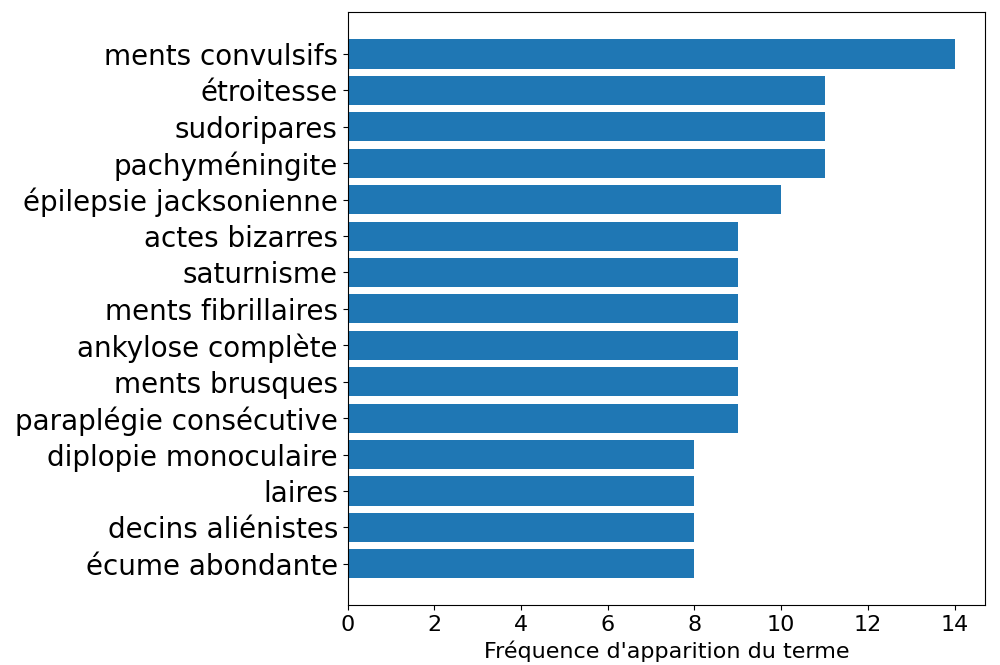
\includegraphics[width=100mm,scale=0.5]{pic/termes_partages.png}
        \caption{Les 15 termes les plus fréquents dans les deux corpus selon \texttt{keyphrase-vectorizers}.}
        \label{fig:enter-label}
    \end{figure}
\end{frame}

%\begin{frame}{Accès à la plateforme technologique \textsc{MeSU}}
%\begin{itemize}
%\item expériences réalisées sur la plateforme \href{https://sacado.sorbonne-universite.fr/}{\textsc{MeSU}} de Sorbonne Université
%\end{itemize}
%\bigskip
%
%Les données et les scripts utilisés dans le cadre de cette étude sont disponibles sur le \href{https://github.com/ljpetkovic/JE\_IA\_HN\_030524}{dépôt GitHub}.
%\end{frame}